\documentclass[conference]{IEEEtran}
\usepackage{cite}
\usepackage{amsmath,amssymb,amsfonts}
\usepackage{algorithmic}
\usepackage{graphicx}
\usepackage{textcomp}
\usepackage{xcolor}
\usepackage{float}
\usepackage{caption}

\graphicspath{{./img2/}{./images/25_50/}{./images/1_25/}}
\begin{document}
\title{COMP90086 Computer Vision Final Project\\
Stereo Disparity
}
\author{
\IEEEauthorblockN{Jun Li Chen}
\IEEEauthorblockA{1043258}
\and
\IEEEauthorblockN{Tianli Cheng}
\IEEEauthorblockA{1128434}
}
\maketitle
\section{Introduction}
Stereo matching is a process of finding correspondence pixels representing the same point in 3-D reality from images taken from different angles and positions. The disparity can be calculated by minus the x coordinate of the right image from the x coordinate of the left image if they are parallel. It is negatively correlated to the depth of the object from the image plane.

Different cost functions exist for similarity computation. This report selects several window-based matching functions and compared their performance over a set of moving vehicle image pairs. Pixels holding the highest similarity will be tagged as correspondences, and the results will be evaluated by computing the root mean square (RMS) between the calculated disparity and the ground truth.
\section{Methodology}
\subsection{Implementation}
Before running each image pair through our program to create a disparity map, a bilateral filter smoothing function is applied to the image pairs. This was done to reduce the effect of noise on our disparity map output. Bilateral filter was chosen as it preserves edges in the image while smoothening the image.

The program iterates through pixels on the left image, while creating a sliding window of search size 25. The sum of absolute difference (SAD) and the sum of square difference (SSD) are selected as the classic similarity measurement functions to start with.

SAD of block W1 and block W2 was calculated by summing up the intensity differences between each corresponding pixel pair, as in:
\begin{equation*}
    SAD=\sum^{n}_{i=0}\sum^{m}_{j=0}|W1[i,j]-W2[i,j]|
\end{equation*}

Similarly, the SSD of block W1 and block W2 was calculated by summing up the square of intensity differences between each corresponding pixel pair, as in:
\begin{equation*}
    SSD=\sum^{n}_{i=0}\sum^{m}_{j=0}(W1[i,j]-W2[i,j])^2
\end{equation*}

SSD is more discriminative compared to SAD since the differences between image patches are amplified by squaring [1]. In case there is one single pixel holding a value that is much larger compared to the rest in the block, SSD will score it higher than SAD does. It means that those pixels holding small differences are more likely to be ignored by SSD.

The pixel index with the lowest difference value in the sliding window to the original pixel on the left image is used as the pixel index to calculate the value of pixel shift as the disparity value for said pixel.
\subsection{Evaluation}
In the output disparity map with a block size of 1 and search size of 25 as shown in Figure 1 below, there are many adjacent areas of high and low disparity, which corresponds to the high RMS value and low pixel error fractions as in Figure 2. This can be caused by noise in the image, or the small search size.

The time taken for SSD and SAD function to complete the disparity map calculation is also very high at around 90--95 seconds for each image.
\begin{figure}[H]
    \centering
    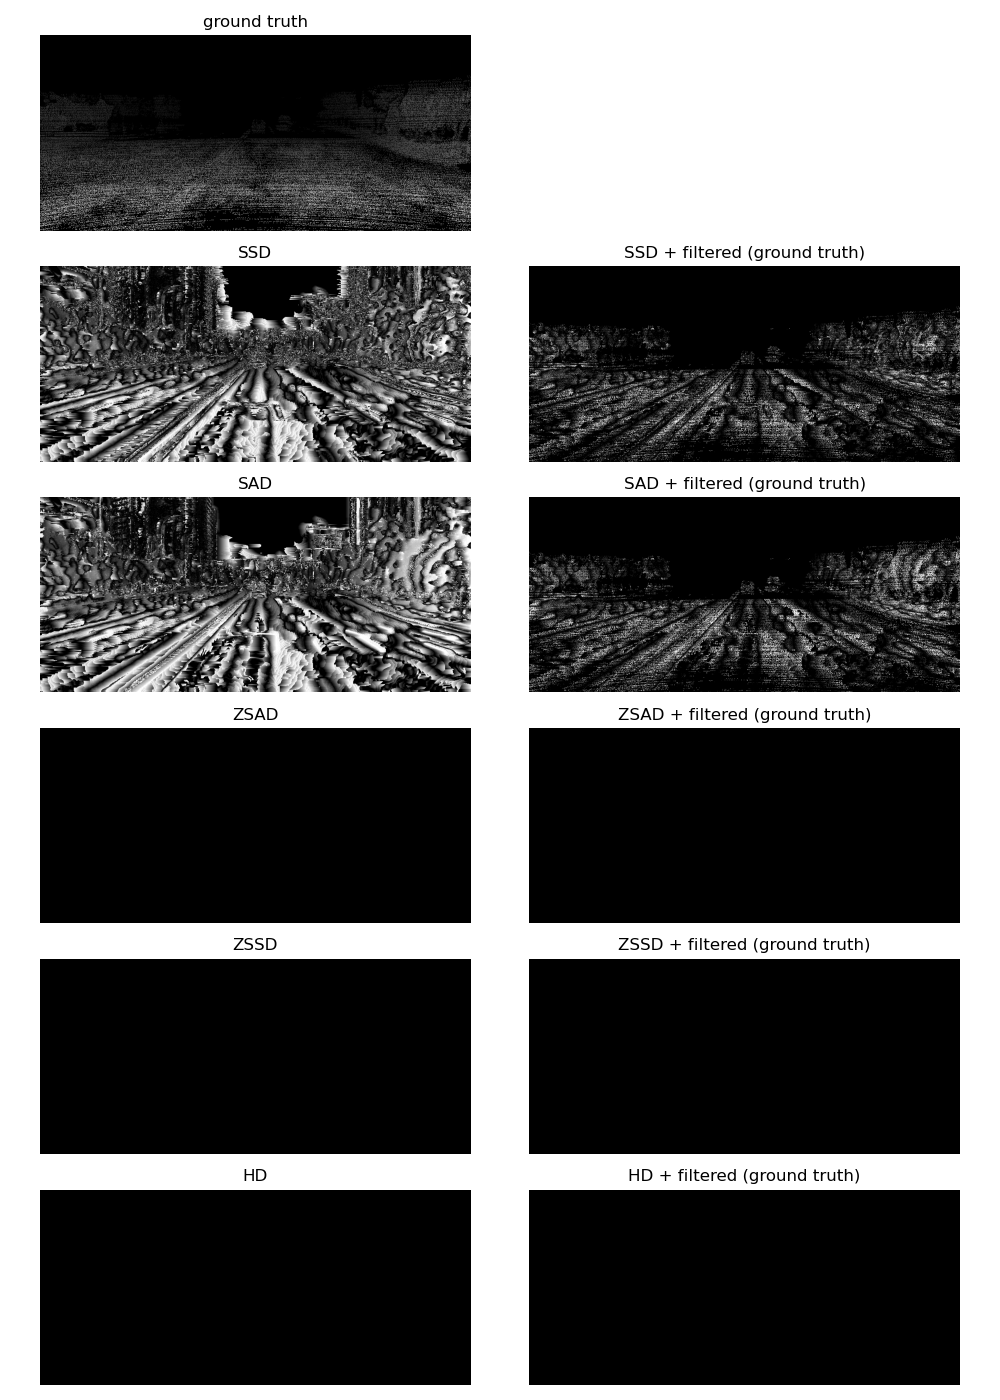
\includegraphics[width=8.8cm]{702_output_1_25.png}
    \captionof{figure}{Disparity map output with block size 1 \& search size 25.}
\end{figure}
\begin{figure}[H]
    \centering
    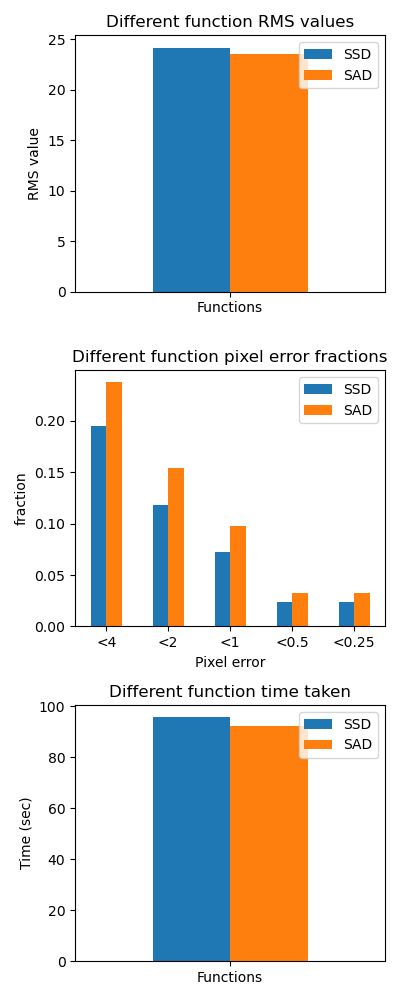
\includegraphics[height=11cm]{702_stats_1_25.png}
    \captionof{figure}{Disparity performance with block size 1 \& search size 25. (See Appendix A for bar chart values)}
\end{figure}
\section{Improvement}
\subsection{Implementation}
Due to the low performance and slow program runtime, the original program was modified to use different comparison functions including ZSAD, ZSSD and HDCT. Furthermore, instead of iterating through each individual pixel to calculate each disparity value, the modified program iterates through a block of size n by n pixels, comparing it to the corresponding sliding window search block of the same size. For example, we used a pixel block size of 25 (width 25, height 25) on the left image, while searching through the right image with a sliding window of size 50 (width 50, height 25). We assume there is no vertical disparity between the image pairs, therefore only the width of the sliding window is varied.

Moreover, three other have been chosen other than SAD and SSD to make a performance comparison in this report. They are zero-mean sum of absolute difference (ZSAD), the zero-mean sum of square difference (ZSSD), and Hamming distance of census transform (HDCT). 

ZSAD and ZSSD, are chosen to perform a certain degree of normalization avoiding the result being biased by large values. ZSAD between blocks is calculated by summing up the deviation differences between each corresponding pixel pair, as in:

\begin{equation*}
    \begin{aligned}
        ZSAD= {} & \sum^{n}_{i=0}\sum^{m}_{j=0}|(W1_{[i,j]}-\frac{1}{nm}\sum^{n}_{i=0}\sum^{m}_{j=0}W1_{[i,j]})\\
        & -(W2_{[i,j]}-\frac{1}{nm}W2_{[i,j]})|
    \end{aligned}
\end{equation*}

It first finds the differences between each element and the mean intensity value in both image blocks, then finds the absolute differences of the corresponding deviation. Similarly, ZSSD was calculated by summing up the square of deviation differences between each corresponding pixel pair, as in:
\begin{equation*}
    \begin{aligned}
        ZSSD= {} & \sum^{n}_{i=0}\sum^{m}_{j=0}((W1_{[i,j]}-\frac{1}{nm}\sum^{n}_{i=0}\sum^{m}_{j=0}W1_{[i,j]})- \\
        & (W2_{[i,j]}-\frac{1}{nm}W2_{[i,j]}))^2
    \end{aligned}
\end{equation*}

By only keeping the deviation, these functions are less sensitive to a general shift in intensity which can be caused by a change in lightning. However, normalization can be taken further by including the relation of a single pixel with the image block it belongs to into consideration. Normalized Cross-Correlation (NCC) is one of the most classic metrics including local relations when mapping similarity between images. It is less sensitive to a linear change in lightning intensity but computationally expensive (D.M. Tsai et al., 2003). Hence, HDCT has been selected as an alternative to NCC and also normalized the image pattern by local correlation. 

The census transform records each pixel holding a lower intensity compared to the center pixel as 0 and the rest as 1. Figure 1 gives an example of how census transform works in a 3 by 3 window.

\begin{figure}[H]
    \centering
    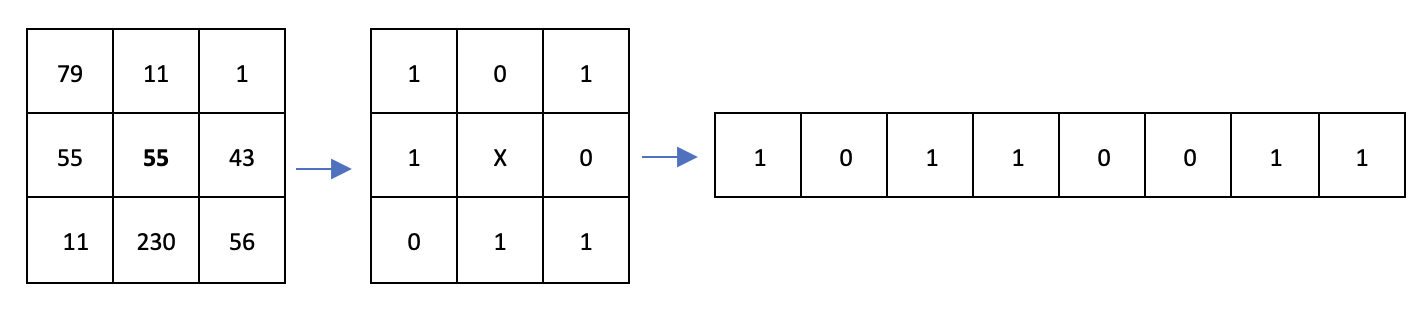
\includegraphics[width=8cm]{fig1.png}
    \caption{Census transform}
\end{figure}

It represents each pixel's relation to the center pixel in a binary form. Therefore, it is non-parametric and insensitive to radiometric variations [2].

The Hamming distance of the census transform between two blocks is calculated by performing a XOR operation on the two 1-D binary representations. By counting the number of 1 existing in the outcome of XOR between blocks, the result represents the number of different patterns. Figure 2 gives an example of how it works.

\begin{figure}[H]
    \centering
    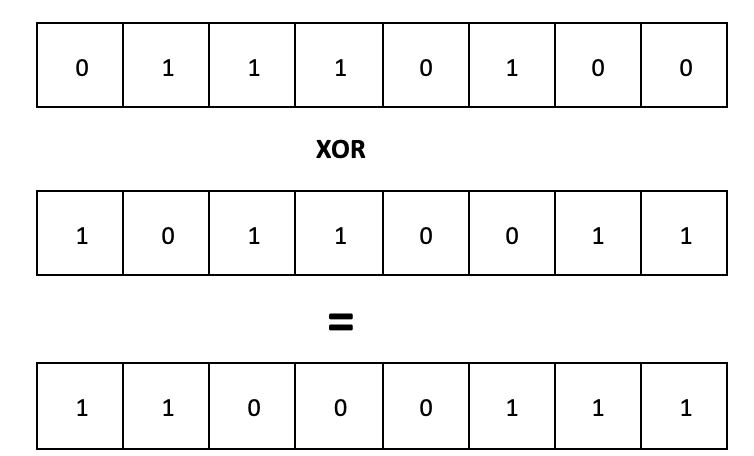
\includegraphics[width=6cm]{fig2.png}
    \caption{Hamming distance of Census transform}
\end{figure}

\subsection{Evaluation}
\begin{figure}[H]
    \centering
    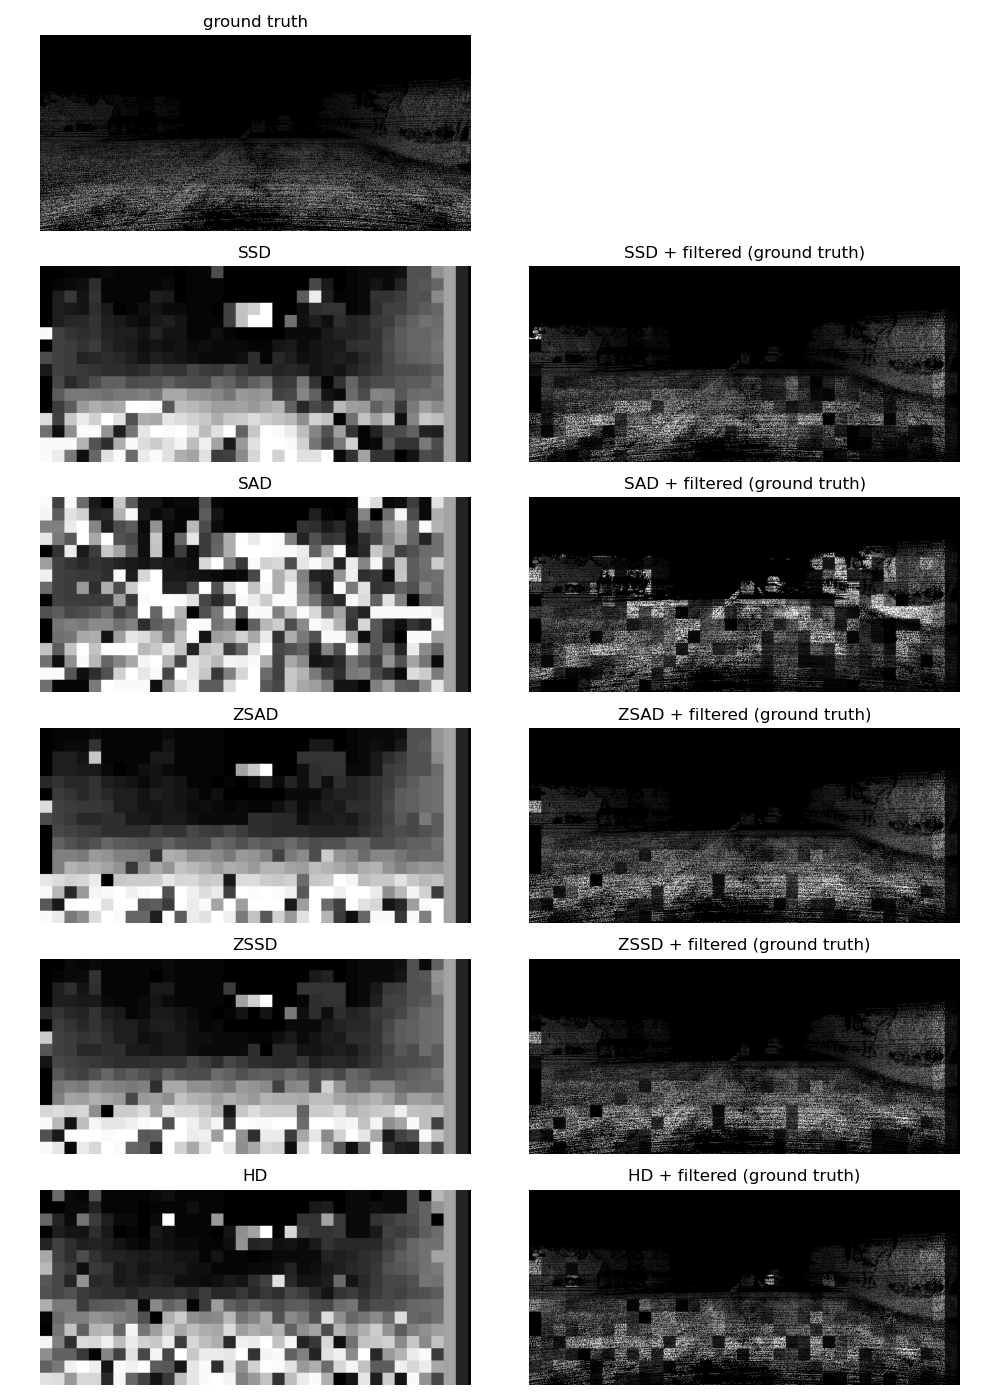
\includegraphics[width=8.8cm]{702_output_25_50.png}
    \captionof{figure}{Disparity map output with block size 25 \& search size 50.}
\end{figure}
\begin{figure}[H]
    \centering
    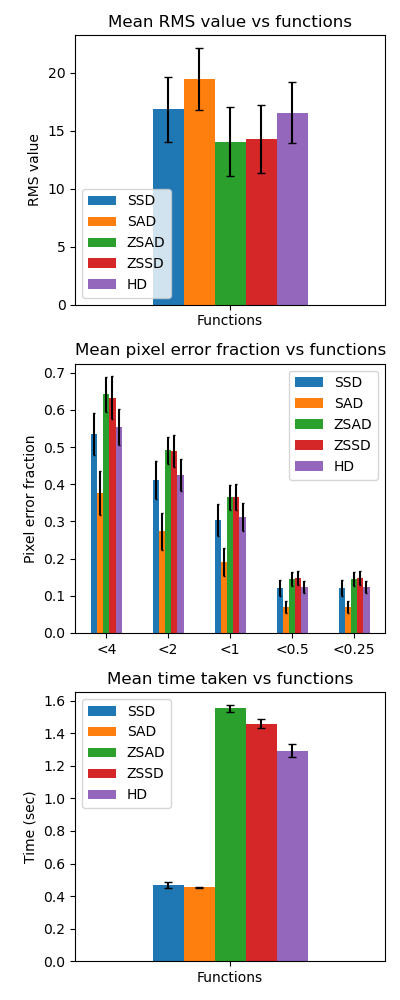
\includegraphics[height=11cm]{stats_25_50.png}
    \captionof{figure}{Disparity performance with block size 25 \& search size 50. (See Appendix A for bar chart values)}
\end{figure}
\section{Analysis}
It is found that the computational time of pixel-wise disparity calculation is extremely long in this case since experiment photos all have 400 by 881 pixels. The function will iterate $400*881*88=31011200$ times if it searches every pixel on the left image and finds correspondence on the right image on the same line. The iteration must be deducted to improve the method's feasibility.

By setting a search size, the program will not iterate over all pixels laying on the same line on the right image but only within a defined searching window of fixed size. Meanwhile, the function will search those image blocks with center coordinates closer to the original coordinate of the block cropped from the left image first, since the correspondence is more likely to be found in those locations.

The number of iterations is further deducted by assuming each pixel in the image block holds the same disparity. By replacing pixel-wise correspondence searching with block-wise correspondence searching, the maximum number of iterations becomes:
\begin{equation*}
    \frac{400*881}{block\_width*block\_height*window\_size}
\end{equation*}

\section{Conclusion}

\newpage
\begin{thebibliography}{00}
\bibitem{1} Schmidt, A., Kraft, M. and Kasiński, A., 2010. An Evaluation of Image Feature Detectors and Descriptors for Robot Navigation. Computer Vision and Graphics, pp.251-259.
\bibitem{2} Sarika, S., Deepambika, V. and Rahman, M., 2015. Census Filtering Based Stereomatching under Varying Radiometric Conditions. Procedia Computer Science, 58, pp.315-320.
\bibitem{3} Tsai, D. and Lin, C., 2003. Fast normalized cross correlation for defect detection. Pattern Recognition Letters, 24(15), pp.2625-2631.
\end{thebibliography}
\vspace{12pt}

\section*{Appendix A}
\begin{center}
    \begin{tabular}{l c c c c c}
        \textbf{Function} & \textbf{SSD} & \textbf{SAD} & \textbf{ZSAD} & \textbf{ZSSD} & \textbf{HD} \\ [0.5ex] 
        Mean & 16.85 & 19.45 & 14.06 & 14.29 & 16.53 \\
        SD & 2.79 & 2.66 & 2.99 & 2.91 & 2.62
    \end{tabular}
    \captionof{table}{RMS statistic table values}
\end{center}
\begin{center}
    \begin{tabular}{l c c c c c}
        \textbf{Function} & \textbf{SSD} & \textbf{SAD} & \textbf{ZSAD} & \textbf{ZSSD} & \textbf{HD} \\ [0.5ex] 
        Mean ($<4$) & 0.536 & 0.376 & 0.642 & 0.634 & 0.555 \\
        Mean ($<2$) & 0.411 & 0.273 & 0.491 & 0.490 & 0.425 \\
        Mean ($<1$) & 0.303 & 0.192 & 0.365 & 0.366 & 0.313 \\
        Mean ($<0.5$) & 0.120 & 0.071 & 0.145 & 0.148 & 0.123 \\
        Mean ($<0.25$) & 0.120 & 0.071 & 0.145 & 0.148 & 0.123 \\
        & & & & & \\
        SD ($<4$) & 0.057 & 0.057 & 0.046 & 0.057 & 0.049 \\
        SD ($<2$) & 0.050 & 0.050 & 0.036 & 0.042 & 0.042 \\
        SD ($<1$) & 0.043 & 0.038 & 0.033 &  0.035 & 0.037 \\
        SD ($<0.5$) & 0.022 & 0.016 & 0.018 & 0.019 & 0.016 \\
        SD ($<0.25$) & 0.022 & 0.016 & 0.018 & 0.019 & 0.016 \\
    \end{tabular}
    \captionof{table}{Pixel error fraction statistic table values}
\end{center}
\begin{center}
    \begin{tabular}{l c c c c c}
        \textbf{Function} & \textbf{SSD} & \textbf{SAD} & \textbf{ZSAD} & \textbf{ZSSD} & \textbf{HD} \\ [0.5ex] 
        Mean & 0.466 & 0.453 & 1.553 & 1.460 & 1.294 \\
        SD & 0.019 & 0.004 & 0.022 & 0.028 & 0.042
    \end{tabular}
    \captionof{table}{Time taken statistic table values}
\end{center}

\end{document}
